        % % Title and author(s)
%%%%%%%%%%%%%%%%%%%%%%%%%%%%%%%%%%%%%%%%%%%%%%%%%%%%%%%
\title{Accelerating Joins with Filters}
\author{Nicholas Corrado \and Xiating Ouyang}
\date{}
%%%%%%%%%%%%%%%%%%%%%%%%%%%%%%%%%%%%%%%%%%%%%%%%%%%%%%%
\documentclass[10pt]{article}
%%%%%%%%%%%%%%%%%%%%%%%%%%%%%%%%%%%%%%%%%%%%%%%%%%%%%%%
% %
% % The next command allows your in import encapsulated
% % postscript files, .epsf or .eps files, which
% % contain vector graphic image data.
% %
%%%%%%%%%%%%%%%%%%%%%%%%%%%%%%%%%%%%%%%%%%%%%%%%%%%%%%%
\usepackage{graphicx}
\usepackage{charter,eulervm}
\usepackage{simpleConference}
%\renewcommand{\baselinestretch}{1.5}
\setcounter{secnumdepth}{3} % default value for 'report' class is "2"
\usepackage{amsthm,amsmath,amssymb,upgreek,marvosym,mathtools}
\usepackage{array}
\usepackage{makeidx}  % allows for indexgeneration
\usepackage{paralist}
\usepackage{subfig}
\usepackage{tabularx}
\usepackage{tabu}
\usepackage{comment}
\usepackage[nottoc]{tocbibind}
\usepackage[usenames,dvipsnames]{color}
\usepackage[pdftex,breaklinks,colorlinks,citecolor={blue}, linkcolor={blue},urlcolor=Maroon]{hyperref}
\usepackage{tkz-graph}
 \linespread{1.25}
\usetikzlibrary{automata, positioning,arrows,shapes,decorations.pathmorphing}

 \tikzset{
->, % makes the edges directed
>=stealth, % makes the arrow heads bold
node distance=3cm, % specifies the minimum distance between two nodes. Change if necessary.
every state/.style={thick, fill=gray!10}, % sets the properties for each ’state’ node
initial text=$ $, % sets the text that appears on the start arrow
}

\newtheorem{theorem}{Theorem}[section]
\newtheorem{lemma}{Lemma}[section]
\newtheorem{reduction}{Reduction}[section]
\newtheorem{proposition}{Proposition}[section]
\newtheorem{scolium}{Scolium}[section]   %% And a not so common one.
\newtheorem{definition}{Definition}[section]
\newtheorem{conjecture}{Conjecture}[section]
\newtheorem{corollary}{Corollary}[section]
%\newenvironment{proof}{{\sc Proof:}}{~\hfill QED}
\newenvironment{AMS}{}{}
\newenvironment{keywords}{}{}
\DeclarePairedDelimiter{\norm}{\lVert}{\rVert}
\newcommand{\todo}{(TO BE CONTINUED...)}
\graphicspath{ {./pics/} }

\newcommand{\paris}[1]{{\color{blue} Paris: [{#1}]}}

\newcommand{\xiating}[1]{{\color{blue} Xiating: [{#1}]}}


\newcommand{\trans}[1]{
	#1^\mathsf{T}
}

\newcommand{\db}{$\mathbf{db}$}
\newcommand{\sjfq}{\texttt{sjfCQA}}
\newcommand{\bcq}{\texttt{bcq}}
\newcommand{\problem}[1]{\textsc{certainty}($#1$)}
\newcommand{\FO}{$\mathbf{FO}$}
\newcommand{\PTIME}{$\mathbf{P}$}
\newcommand{\LSPACE}{$\mathbf{L}$}
\newcommand{\coNP}{$\mathbf{coNP}$}
\newcommand{\und}[1]{\underline{#1}}
\newcommand{\NL}{$\mathbf{NL}$}
\newcommand{\JOIN}{\bowtie}

\begin{document}
\newpage
\maketitle


\abstract{In query optimization on star schemas, lookahead information passing (LIP) is a strategy exploiting the efficiency of probing succinct filters to eliminate practically all facts that do not appear in the final join results before performing the actual join. Assuming data independency across all columns in the fact table, LIP achieves efficient and robust query optimization. We present LIP-$k$, a variant of LIP that only remembers the hit/miss statistics for the previous $k$ batches, achieving empirically efficient query execution on fact table with correlated and even adversarial data columns. We implemented LIP and LIP-$k$ on a skeleton database on top of Apache Arrow and analyze the performance of each variant of LIP using the notion of competitive ratio in online algorithms.}


\section{Introduction}

Performing join operations in database management systems is a fundamental and prevalent task in the modern data industry. Continuous efforts have been spent on building a reliable query optimizer over the last few decades. However, the current optimizers may still produce disastrously inefficient query plans which involves processing unnecessarily gigantic intermediate tables \cite{leis2015good,rabl2013variations}. The \textit{Lookahead Information Passing (LIP)} strategy aggressively uses Bloom Filters to filter the fact tables, effectively reducing the sizes of the intermediate tables. LIP is provably as efficient and robust as computing the join using the optimal query plan \cite{zhu2017looking}. The key idea behind LIP is to estimate the filter selectivity of each dimension table and adaptively reorder the sequence of applying the filters to the fact table. 


The filtering process can be modeled as the \textsc{LIP} problem in an online setting: Suppose we fix $n$ filters, and the tuples in the fact table arrives in an online fashion. Upon arrival of each tuple, one has to decide a sequence of filters to probe the tuple, with an objective of minimizing the number of probes needed to decide whether to accept the tuple and forward it to the hash join phase, or to eliminate it. A mechanism deciding the sequence of applying the filters is thus crucial to the success of LIP. If a tuple passes all filters, \textit{all} mechanisms must probe the tuple to all $n$ filters to confirm its passage. If a tuple is eliminated by at least one filter, then the \textit{optimal} mechanism would apply any filter that rejects the tuple first, using only one probe. Thus, given any fact table $F$, the number of probes that an optimal mechanism requires to process all tuples in the fact table can be readily computed: 
\[
	\textsc{OPT}(F) = n|F_{\text{pass}}| + |F_{\text{reject}}|,
\]
where $|F_{\text{pass}}|$ and $|F_{\text{reject}}|$ are the number of tuples in $F$ that pass all filters and are rejected in $F$ respectively. For any mechanism $\mathcal{M}$, denoted by \textsc{ALG}$_{\mathcal{M}}(F)$ the number of probes that $\mathcal{M}$ performed to process all tuples in the fact table.  The performance of any mechanism $\mathcal{M}$ can thus be measured by 
\[
	\max_{F}\frac{\textsc{ALG}_{\mathcal{M}}(F)}{\textsc{OPT}(F)},
\]
called the \textit{competitive ratio} of $\mathcal{M}$. The competitive ratio is always at least 1 by definition, and in this problem the competitive ratio is at most $n$, the number of filters, since one mechanism can probe each tuple to at most $n$ filters.


This project aims at designing efficient LIP mechanisms and measure their performance in terms of their overall running time and competitive ratio. We will build a skeleton database system on top of Apache Arrow supporting LIP and hash-joins to conduct our experiments and test the performance of our variant LIP mechanisms against the hash-join and the orignal LIP. We also present a theoretical result showing that no deterministic mechanism can have a competitive ratio better than $n$, and discuss possible extensions of LIP to use randomness to design a better mechanism.


%Experimental results show that as LIP uses more filters, the increase in performance improvement diminishes, displaying a concave curve. One reason is that if the cache cannot hold all filters, then evicting the filters causes significant overhead in the performance. Moreover, when probing each fact tuple against all filters, the more selective filters are inserted to cache first. When the cache is full, the cache manager has to evict a more selective filter so that a less selective filter can be inserted to cache. Once LIP switches to probing the next fact tuple, the more selective filter is inserted into the cache again, while one could have skipped probing against certain inselective filters to reduce the replacement overhead.


%This project aims at investigating the effect of skipping certain LIP filter on improving the performance of LIP, and if possible, derive a theoretical guarantee on the performance of LIP against the optimal joining sequence. We will build a skeleton database system on top of Apache Arrow supporting LIP and hash-joins to conduct our experiments and test the performance of our revised LIP strategy against the hash-join.



\section{Lookahead Information Passing (LIP)}
In this section, we first present the LIP strategy in \cite{zhu2017looking}, and then discuss our variant LIP-$k$, designed to respond to local skewness more quickly than LIP. Finally, we discuss the competitive ratios of all deterministic mechanisms and provide proof on its lower bound. Some possible extensions of LIP using randomness is also discussed.



\subsection{LIP}
The LIP strategy has three stages: (1) Building a hash table and a filter for each dimension table, (2) probe each fact tuple on the filters, producing a set of fact tuples with false positives, and (3) probe the hash table of each dimension table to eliminate the false positives. In what follows we mainly discuss stage (2) since stages (1) and (3) are readily implemented by either the database engine or the filter constructors.

Let $F$ be the fact table and $D_i$ the dimension tables for $1 \leq i \leq n$. We denote the number of facts in $F$ and each $D_i$ as $|F|$ and $|D_i|$. A LIP filter on $D_i$ is implemented using a Bloom filter, with false positive rate $\varepsilon$. The true selectivity $\sigma_i$ of $D_i$ on fact table $F$ is given by $\sigma_i = |D_i \JOIN_{pk_i = fk_i} F| / |F|,$ where $pk_i$ is the primary key of $D_i$ and $fk_i$ is the foreign key of $D_i$ in $F$. The \texttt{LIP-join} algorithm, depicted in Figure \ref{fig:lip}, computes the indices of tuples in $F$ that pass the filtering of each Bloom filter of $D_i$. Note that there is an innate false positive rate $\varepsilon$ associated with each Bloom Filter, and thus the set of indices is a superset of the true set of indices of tuples appearing in the final join result.

The partition in \cite{zhu2017looking} satisfies that $|F_{t+1}| = 2|F_{t}|$ at line 5, and the algorithm approximates the true selectiveness $\sigma_i$ of each dimension $D_i$ using $pass[i]/count[i]$, the aggregated selectiveness since the beginning.

\begin{figure*}[h!]
	\centering
	\tikz\path (0,0) node[draw, text width=.8\textwidth, rectangle, inner xsep=20pt, inner ysep=10pt]{
		\begin{minipage}[t!]{\textwidth}
			{\sc Procedure}: \texttt{LIP-join}
			\\
			{\sc Input}: a fact table $F$ and a set of $n$ Bloom filters $f_i$ for each $D_i$ with $1 \leq i \leq n$
 			\\
			{\sc Output}: Indices of tuples in $F$ that pass the filtering
			\begin{tabbing}
				Aaa\=aaA\=Aaa\=Aaa\=Aaa\=AAAAAAAAAAAAAAAAAAAAAAAAA\=A \kill
				1.\> Initialize $I = \emptyset$
				\\
				2.\> {\bf foreach } filter $f$ {\bf do}
				\\
				3.\>\> $count[f] \leftarrow 0$
				\\
				4.\>\> $pass[f] \leftarrow 0$ 
				\\
				5.\> Partition $F = \bigcup_{1 \leq t \leq T}F_t$. 
				\\
				6.\> {\bf foreach } fact block $F_t$ {\bf do} 
				\\
				7.\>\> {\bf foreach } filter $f$ in order {\bf do}
				\\
				8.\>\>\> {\bf foreach} index $j \in F_t$ {\bf do}
				\\
				9.\>\>\>\> $count[f] \leftarrow count[f] + 1$
				\\
				10.\>\>\>\> {\bf if }$f$ contains $F_t[j]$ 
				\\
				11.\>\>\>\>\> $I \leftarrow I \cup \{j\}$ 
				\\
				12.\>\>\>\>\> $pass[f] \leftarrow pass[f] + 1$
				\\
				13.\>\> {\bf sort} filters $f$ in nondesending order of $pass[f]/count[f]$
				\\
				14.\> {\bf return } $I$
			\end{tabbing}  
		\end{minipage}
	};
	\caption{The LIP algorithm for computing the joins.}
	\label{fig:lip}
\end{figure*}


\subsection{LIP-$k$}

LIP strategy in Figure \ref{fig:lip} estimates the selectivity of each filter using statistics from the beginning batch, which is inefficient for certain distribution or physical layout of data. Consider some filter $f$ that is very selective for the first $t_0$ iterations at line 6 and not selective for the remaining iterations. (For example, a filter $f$ filtering for \texttt{year} $\geq 2017$ and the \texttt{Date} table is sorted in \texttt{year}.) In this case, LIP would obtain a good estimate of the selectivity of $f$ during the first $t_0$ iterations, and thus tend to apply $f$ early in the remaining iterations. However, it is more efficient to postpone applying $f$ in the remaining iterations, despite $f$ has good selectivity in the first $t_0$ iterations. One remedy to this is to only ``remember" the hit/miss statistics of each filter over the previous $k$ batches.

\begin{figure*}[h!]
	\centering
	\tikz\path (0,0) node[draw, text width=.8\textwidth, rectangle, inner xsep=20pt, inner ysep=10pt]{
		\begin{minipage}[t!]{\textwidth}
			{\sc Procedure}: \texttt{LIP-$k$}
			\\
			{\sc Input}: a fact table $F$ and a set of $n$ Bloom filters $f_i$ for each $D_i$ with $1 \leq i \leq n$
 			\\
			{\sc Output}: Indices of tuples in $F$ that pass the filtering
			\begin{tabbing}
				Aaa\=aaA\=Aaa\=Aaa\=Aaa\=AAAAAAAAAAAAAAAAAAAAAAAAA\=A \kill
				1.\> Initialize $I = \emptyset$
				\\
				2.\> {\bf foreach } filter $f$ {\bf do}
				\\
				3.\>\> Initialize $count[f] \leftarrow 0$, $pass[f] \leftarrow 0$ 
				\\
				4.\>\> Initialize $count\_queue[f]$ with $k$ zeros and $pass\_queue[f]$ with $k$ zeros.
				\\
				5.\> Partition $F = \bigcup_{1 \leq t \leq T}F_t$. 
				\\
				6.\> {\bf foreach } fact block $F_t$ {\bf do} 
				\\
				7.\>\> {\bf foreach } filter $f$ in order {\bf do}
				\\
				8.\>\>\> {\bf foreach} index $j \in F_t$ {\bf do}
				\\
				9.\>\>\>\> $count[f] \leftarrow count[f] + 1$
				\\
				10.\>\>\>\> {\bf if }$f$ contains $F_t[j]$ 
				\\
				11.\>\>\>\>\> $I \leftarrow I \cup \{j\}$ 
				\\
				12.\>\>\>\>\> $pass[f] \leftarrow pass[f] + 1$
				\\
				13.\>\>\> $count\_queue[f].dequeue()$ and $pass\_queue[f].dequeue()$
				\\
				14.\>\>\> $count\_queue[f].enqueue(count[f])$ and $pass\_queue[f].enqueue(pass[f])$
				\\
				15.\>\>\> Reset $count[f] \leftarrow 0$, $pass[f] \leftarrow 0$ 
				\\
				16.\>\> {\bf sort} filters $f$ in nondesending order of $sum(pass\_queue[f])/sum(count\_queue[f])$
				\\
				17.\> {\bf return } $I$
			\end{tabbing}  
		\end{minipage}
	};
	\caption{The LIP algorithm for computing the joins.}
	\label{fig:lip-k}
\end{figure*}

Empirical data shows that for the orignal SSB dataset and certain queries, LIP-$k$ is as fast as LIP, and for certain datasets and queries LIP-$k$ is faster than LIP. Detailed empirical data are presented and analyzed in Section \ref{sec:experiment}.



\subsection{Competitive Ratio Analysis}

The LIP strategy and its variant LIP-$k$ depicted in Figure \ref{fig:lip} and \ref{fig:lip-k} are \textit{deterministic}, i.e.\ multiple executions over the same fact table would produce the same result. Experimental results show that LIP performs almost optimally compared to the performance of hash join in the optimal sequence \cite{zhu2017looking} on the benchmark dataset, in which the keys are distributed almost uniformly. However, it can be shown that deterministic mechanism in the worst case can never achieve a competitive ratio less than $n$, when played against an adversary producing an adversarial dataset.


\begin{theorem}
	Let $n$ be the number of filters in the LIP problem. There is no deterministic mechanism $\mathcal{M}$ achieving a competitive ratio less than $n$ for the \textsc{LIP} problem.
\end{theorem}

\begin{proof}
	We present an adversary to the mechanism $\mathcal{M}$ such that $\mathcal{M}$ only achieves a competitive ratio of $n$ in the worst case. Let the $n$ filters be $f_1, f_2, \dots, f_n$ and consider $n$ tuples $t_1, t_2, \dots, t_n$, where $t_i \notin f_i$ but $t_i \in f_j$ for any $i \neq j$.

	The adversary proceeds as follows: It first observes the sequence of filters $\sigma_t$ at any step $t$ set by the mechanism $\mathcal{M}$, and produce the input $f_{\sigma_t(n)}$ to the mechanism $\mathcal{M}$. Thus the mechanism $\mathcal{M}$ would require $n$ filter probes to eliminate $f_{\sigma_t(n)}$ at each step $t$, whereas the optimal sequence is to apply $\sigma_t(n)$ at the first place. Thus it yields a competitive ratio of $n$.
\end{proof}


It might be possible to design a randomized mechanism $\mathcal{M_p}$ that can achieve a better competitive ratio than $n$. The randomized mechanism would, at the end of each batch, select a sequence of applying the filters from a distribution of all filter permutations, based on the estimated selectivities. However, we have not obtained any algorithmic upper bound on the competitive ratio.  


In the practical perspective however, one wishes to minimize the total running time of the mechanism $\mathcal{M}$, which is effectively the sum of the running time of the mechanism and the running time of building the filters and performing the probes. A trade-off between having a near optimal mechanism that consumes much time and allowing many failed probes to eliminate each non-participating tuple is therefore of much interest. 





\section{Database Implementation}

We have developed a prototype database system supporting basic select and join operations on top of Apache Arrow \cite{apachearrow}, a column-store format. This minimal prototype is sufficient to benchmark the performance of our Hash join, LIP, and LIP-$k$.

Our implementations of LIP and LIP-k only support left-deep join tree plans where the fact table is the ``outer table" in every join. We assume that the fact table schema contains foreign keys to all dimension tables, and each dimension table is single-key. Given a star schema fact table $F$ and dimension tables $D_i$ for $1 \leq i \leq n$, a join query in our system specifies selectors $\sigma_F$ for $F$ and $\sigma_i$ for each $D_i$, and executing that query will return 

$$\sigma_F(F) \JOIN \sigma_1(D_1) \JOIN \dots \JOIN \sigma_n(D_n)$$

\noindent projected on the schema of $F$, {\it i.e.}~we output the tuples in $F$ that can be joined with each $D_i$. The supported primitive selectors allow for selection ($=, \leq, \geq, <, >$) on scalar values and ranges. Range selections are executed using \texttt{BETWEEN} ($\ell$, $h$), which selects all $x$ with $\ell \leq x \leq h$. 

The selectors for each dimension can be either a primitive selector consisting of simple predicate ({\it e.g.} \texttt{ORDER DATE} = 1997) 
or a composition (logical AND/OR) of multiple primitive/composite selectors. 
This is implemented using the Composite design pattern.
Apache Arrow does not yet support vectorized string comparison operations nor vectorized range comparison operations.
For queries involving string and/or range selections, 
we instead scan along the column, checking which rows satisfy the selection predicate. 
Such selections are inherently slower than the supported vectorized selections. 
Because all of our join implementations must implement row-wise selection for string and range predicates, 
all algorithms suffer the same slowdown. 
Thus, this implementation caveat does not preclude us from studying the relative performance of LIP and LIP-$k$.

We only support string and numeric data types. All numeric data is stored an 64-bit integers by default.

The hash join algorithm first produces a hash table $T_i$ for each $\sigma_i(D_i)$, projected on the $k_i$, and then probe each tuple in the fact table against all $T_i$. We used Sparseepp (accessible at \url{https://github.com/greg7mdp/sparsepp}) as our implementation of the hash table, in which the sparsehash by Google (accessible at \url{https://github.com/sparsehash/sparsehash}) is used as the underlying hash function. All primary keys are regarded as 64-bit integers.

For LIP and LIP-$k$, the succinct filter structure we choose is the Bloom filters. 
The default false-positive rate is set to 0.001, which requires 10 hash functions.
We use Knuth's Multiplicative hash function, extended to accept a 64-bit integer as a seed. 
Our minimal implementation does not support selectivity estimation, 
so we initialize each Bloom filter assuming $\sigma(D_i) = \frac{1}{2}$, 
{\it i.e.} assuming half of the keys in each dimension table will be inserted into the filter.

Our code is available at \url{https://github.com/NicholasCorrado/CS764}.




\section{Empirical Results}\label{sec:experiment}

In this section we present the empirical results obtained from running Hash-join, LIP and LIP-$k$ on several datasets. In Section \ref{sec:dataset}, we present the datasets we use and describe how we generate skewed and adversarial datasets. In Section \ref{sec:time} we present the running time of multiple strategies and discuss their performance. In Section \ref{sec:ratio} we discuss how $k$ affects the competitive ratio of LIP-$k$ empirically on our datasets.

\subsection{Datasets}
\label{sec:dataset}

The Star Schema Benchmark (SSB) is a variation of the TPC-H benchmark 
consisting of a large central fact table \texttt{LINEORDER} and four smaller dimension tables (\texttt{DATE}, \texttt{PART}, \texttt{CUSTOMER}, and \texttt{SUPPLIER}).
The benchmark has 13 select-project-join queries split across four groups. 
We generate all tables in the benchmark using the SSB generator found at \url{https://github.com/UWQuickstep/SQL-benchmark-data-generator/tree/master/ssbgen}.
We refer the \texttt{LINEORDER} table produced from the SBB generator with SF = 1 as \texttt{LINEORDER-UNIFORM}, 
since it's foreign keys for each tuple are sampled from a uniform distribution of possible keys ({\it i.e.} there is no skew).

We modify the \texttt{LINEORDER-UNIFORM} table to produce four additional skewed \texttt{LINEORDER} tables.
For simplicity in generating skew tables, we skew the \texttt{ORDER DATE} foreign key in the origin \texttt{LINEORDER} table, corresponding to the primary key of the \texttt{DATE} table. 
We alter the distribution of \texttt{ORDER DATE} foreign keys satisfying \texttt{DATE.YEAR = 1997 OR DATE.YEAR = 1998}, which we shorten to \texttt{SKEW PRED}.
The skewed tables are as follows:


\begin{itemize}
    \item \texttt{LINEORDER-DATE-FIRST-HALF}: Let $N$ be the total number of batches in \texttt{LINEORDER}. 
    The first $N/2$ batches have $\sigma_{\texttt{SKEW PRED}} = 1$ while the remaining $N/2$ batches have $\sigma_{\texttt{SKEW PRED}} = 0$.
    In other words, The first $N/2$ batches contain only keys satisfying \texttt{SKEW PRED}, 
    while the next $N/2$ batches contain only keys not satisying \texttt{SKEW PRED}, 
    and so on. 

    \item \texttt{LINEORDER-DATE-50-50}: The first 50 batches have $\sigma_{\texttt{SKEW PRED}} = 1$ while the next 50 batches have $\sigma_{\texttt{SKEW PRED}} = 0$, and so on.

    \item \texttt{LINEORDER-DATE-LINEAR}: $\sigma_{\texttt{SKEW PRED}}$ increases linearly from 0 to 1 across the \texttt{LINEORDER} table, 
    {\it i.e.} batch $k$ has $\sigma_{\texttt{SKEW PRED}} = k/N$.

    \item \texttt{LINEORDER-DATE-PART-ADVERSARY}: We defer discussion on this dataset to Section~\ref{sec:ratio}, 
    as it requires a careful description of its construction.

\end{itemize} 


All datasets are summarized in Table~\ref{tab:skew_datasets}. All datasets use the same dimension tables originally produced from the SSB generator with SF = 1.

\begin{table}
\begin{center}
\begin{tabular}{ |>{\ttfamily}l|>{\ttfamily}c|l| } 
\hline
{\bf Dataset Name} & {\bf Skewed Foreign Keys} & {\bf Description of Skew} \\
\hline
\hline
LINEORDER-UNIFORM& N/A & No skew. Generated from SSB data generator\\
& & with SF = 1.\\
\hline
LINEORDER-DATE-FIRST-HALF& ORDER DATE & $\sigma_{\texttt{SKEW PRED}}$ changes from 1 to 0 halfway through\\
& &  the table.\\
\hline
LINEORDER-DATE-50-50& ORDER DATE & $\sigma_{\texttt{SKEW PRED}}$ changes from 1 to 0 or from 0 to 1 \\
& & every 50 batches. \\ 
\hline
LINEORDER-DATE-LINEAR& ORDER DATE & $\sigma_{\texttt{SKEW PRED}}$ increases linearly from 0 to 1 \\
& & through the table. \\
\hline
LINEORDER-DATE-PART-ADVERSARY& ORDER DATE & See Section~\ref{sec:ratio}\\
& PART KEY & \\
\hline

\end{tabular}
\end{center}

\caption{Brief descriptions of all datasets studied.}
\label{tab:skew_datasets}
\end{table}

\subsection{Execution Time}
\label{sec:time}

\begin{figure}
    \centering
    \subfloat[]{
        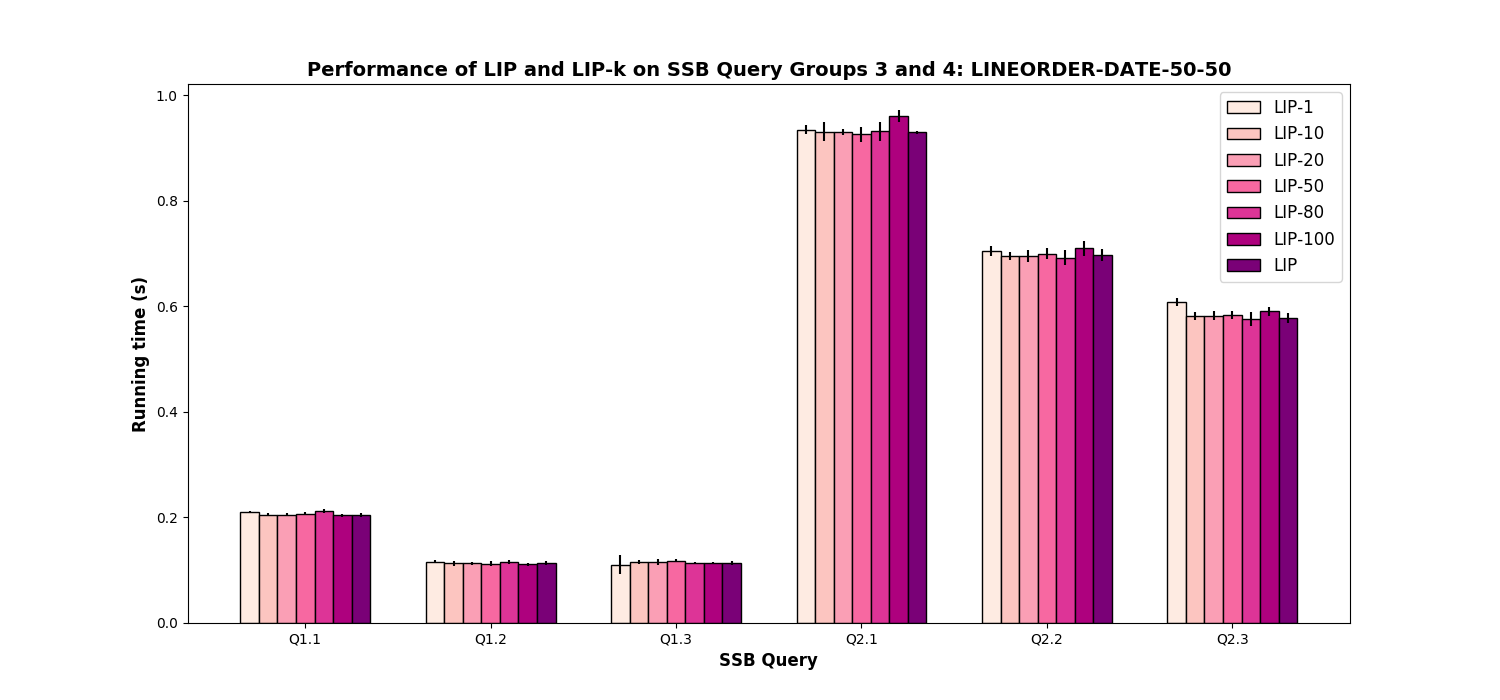
\includegraphics[width=0.9\textwidth,keepaspectratio]{lip-and-lipk-date-50-50-q1-q2}

    }\\
    \subfloat[]{
        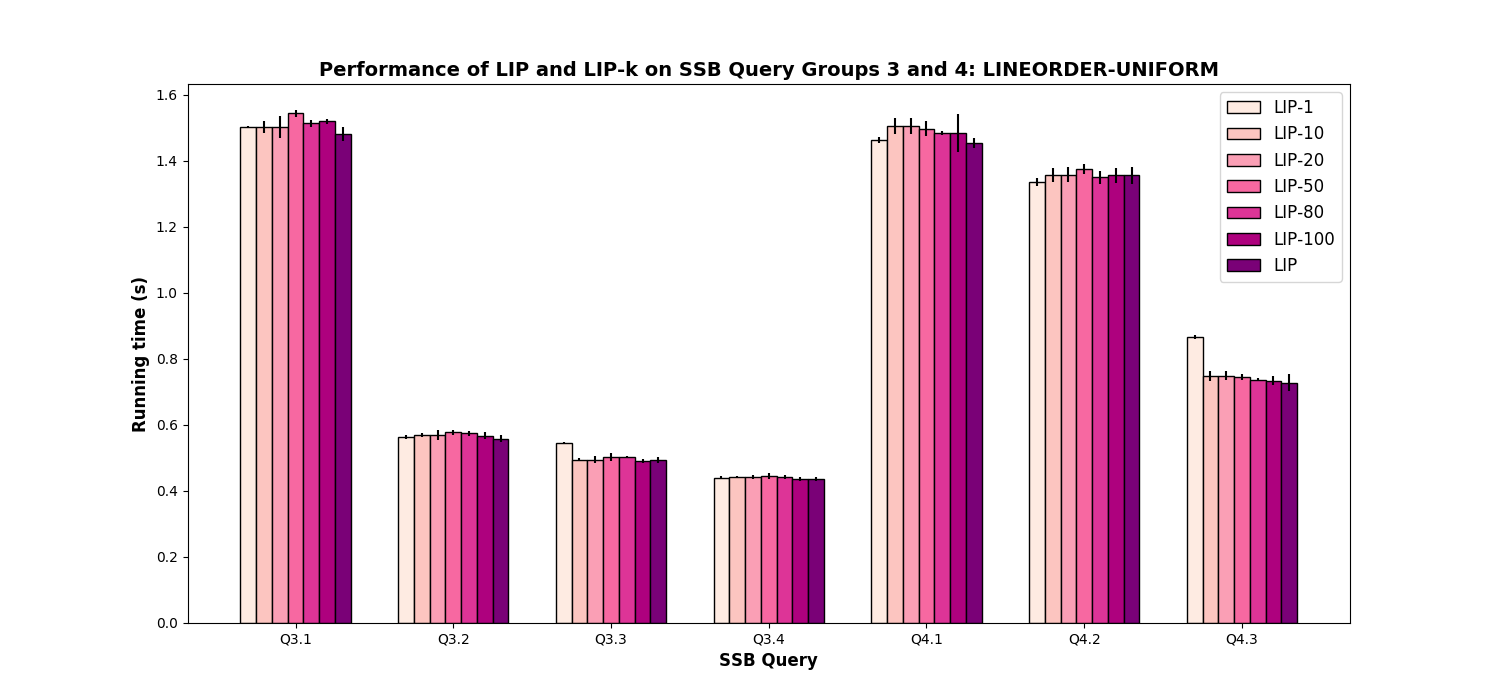
\includegraphics[width=0.9\textwidth,keepaspectratio]{lip-and-lipk-uniform}
    }
    \caption{Execution time for SSB query groups 1 and 2 on (a) \texttt{LINEORDER-DATE-50-50} and query group 3 and 4 on (b)~\texttt{LINEORDER-UNIFORM}}
    \label{fig:times0}
\end{figure}

\begin{figure}
    \centering
    \subfloat[]{
        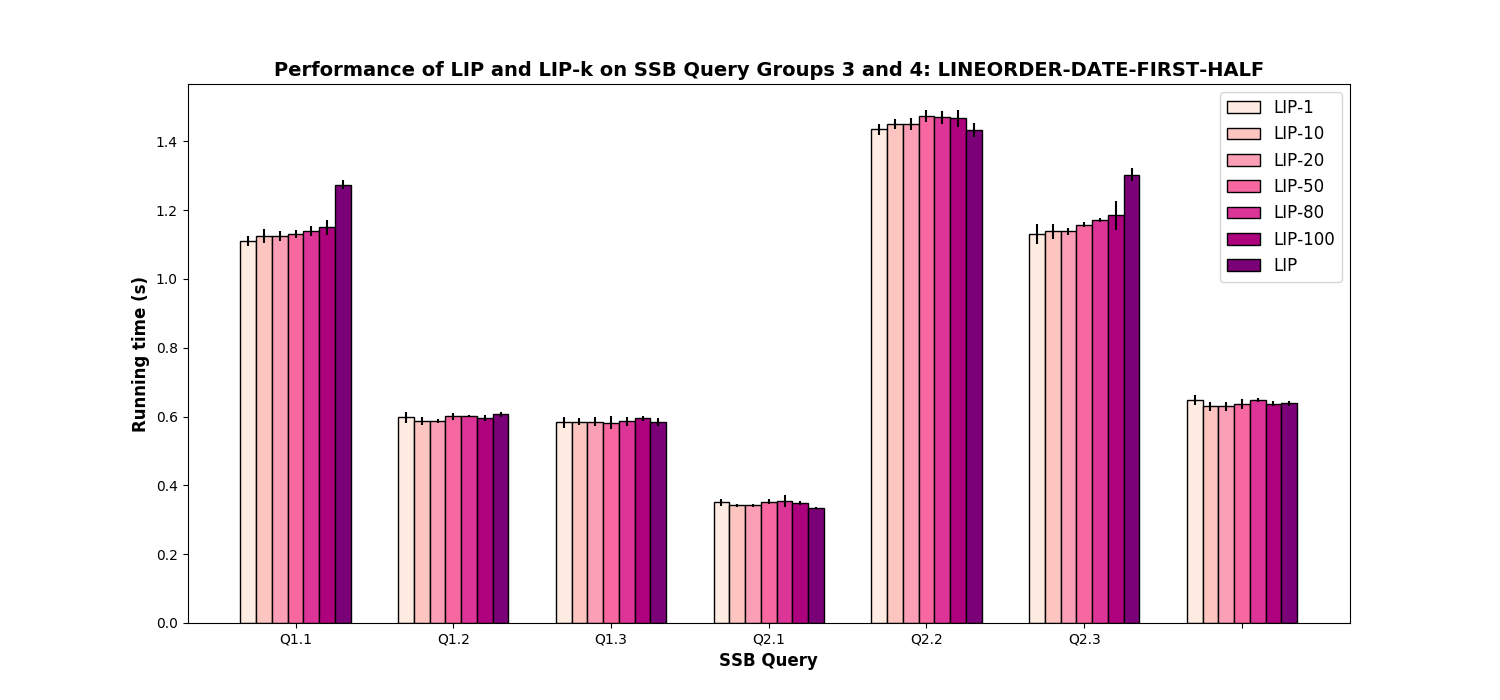
\includegraphics[width=0.9\textwidth,keepaspectratio]{lip-and-lipk-date-first-half}
    }\\
    \subfloat[]{
        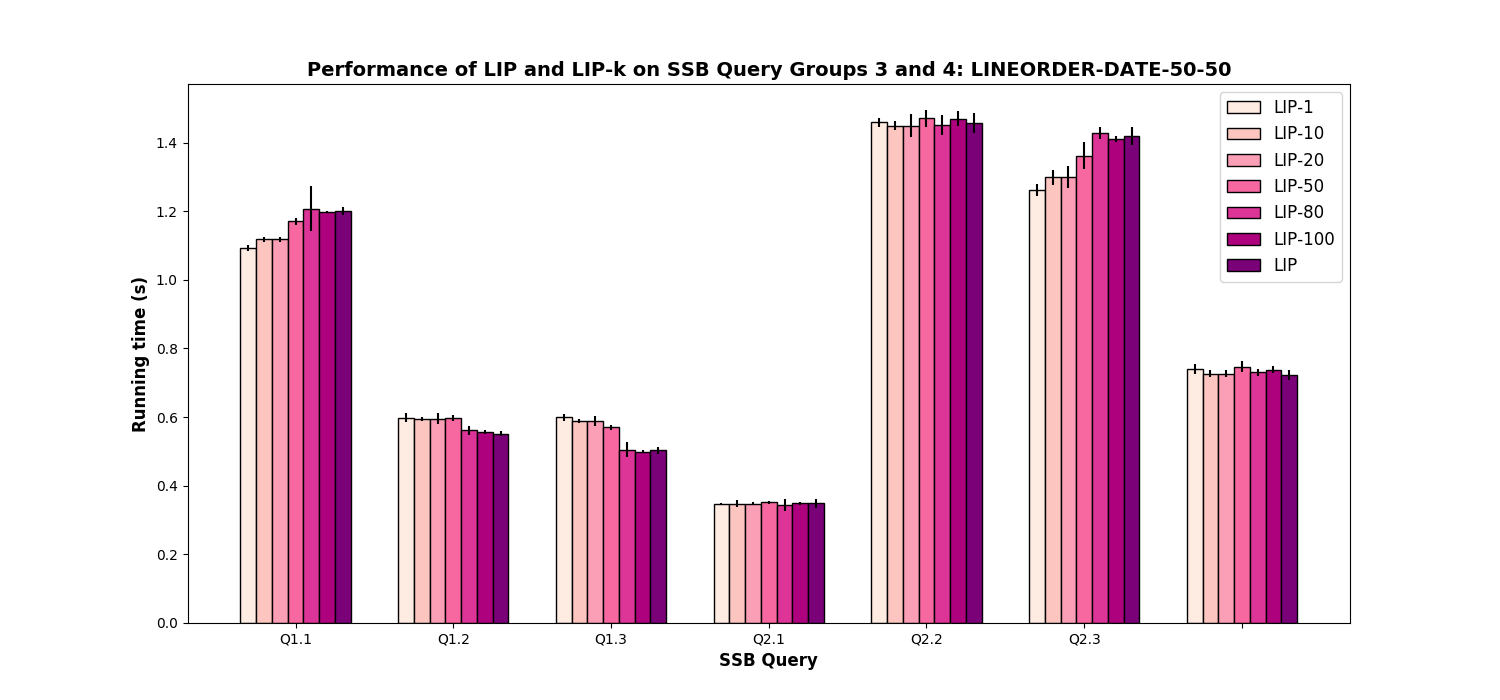
\includegraphics[width=0.9\textwidth,keepaspectratio]{lip-and-lipk-date-50-50}
    }
    \caption{Execution time for SSB query groups 3 and 4 on (a) \texttt{LINEORDER-DATE-FIRST-HALF} and (b)~\texttt{LINEORDER-DATE-50-50}}
    \label{fig:times1}
\end{figure}


\begin{figure}
    \centering    
    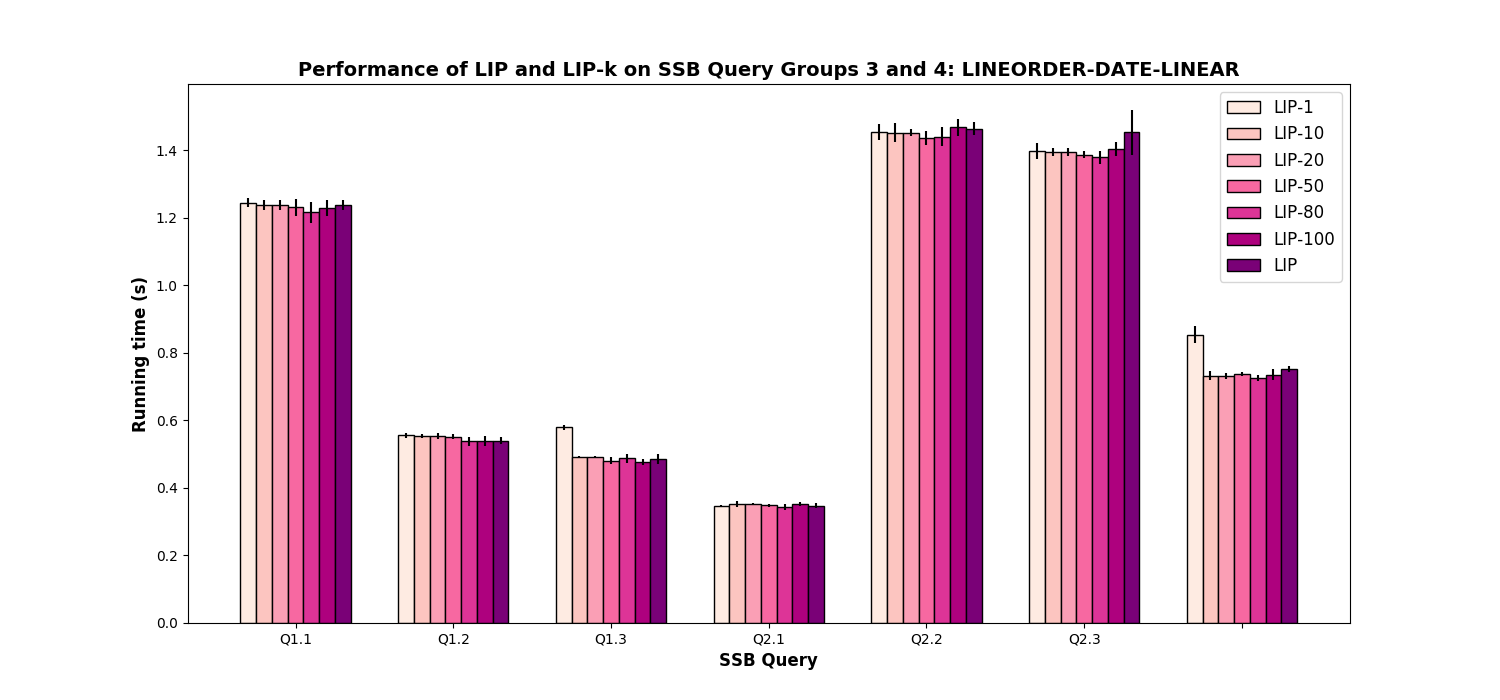
\includegraphics[width=0.9\textwidth,keepaspectratio]{lip-and-lipk-date-linear}
    \caption{Execution time for SSB query groups 3 and 4 on \texttt{LINEORDER-DATE-LINEAR}}
    \label{fig:times2}
\end{figure}

SSB query groups 1 and 2 do not join on \texttt{ORDER DATE}, 
and thus their execution times are unaffected by the skewed key column. 
Fig.~\ref{fig:times0}(a) shows execution times for these queries on the \texttt{LINEORDER-DATE-50-50} table.
As expected, we observe that LIP and LIP-$k$ have roughly equal performance for these queries.
Henceforth, we will exclude query groups 1 and 2 from our analysis, 
as they provide us no insight into the relative performance of LIP and LIP-$k$. 
Nevertheless, from these results, we see that the extra overhead associated with LIP-$k$ is negligible.

Query groups 3 and 4 --- except for query 4.1 --- join on \texttt{ORDER DATE}, 
so our skew can potentially affect the execution of LIP and LIP-$k$ on these queries.
Thus, we include only queries from groups 3 and 4 in our analysis. 
Query 4.1 is included as a "sanity check", since LIP and LIP-$k$ should have roughly equal performance on this query.

Fig.~\ref{fig:times0}(a) shows execution times for these queries on the \texttt{LINEORDER-UNIFORM} table.
We see that LIP-$1$ performs worse than all other algorithms on queries 3.3 and 4.3.
because it does not compute an accurate selectivity estimate using only one previous batch.
Otherwise, there is little difference between LIP and LIP-$k$ on uniform data.

Fig.~\ref{fig:times1}(a) shows execution times using \texttt{LINEORDER-DATE-FIRST-HALF}. 
We see that LIP and LIP-$k$ have roughly equal performance on queries 3.2, 3.3, 3.4, and 4.3 (in addition to 4.1).
In such queries, we do not gain much by responding to local changes in the key distribution,
since there exists another filter, {\it e.g.} the \texttt{SUPPLIER} filter, that is very selective. 
LIP generally will not notice when $\sigma_i^{\texttt{DATE}} = 0$ 
and instead applies the \texttt{SUPPLIER} filter first.
We observe that it is ``good enough" to apply a very selective filter first, even if it is not optimal.
On the other hand, LIP-$k$ performs better on queries 3.1 and 4.2, 
since the other filters in these queries are not particularly selective. 
We also observe that smaller $k$ has slightly better performance, 
because small $k$ can respond much more quickly to the sudden change in selectivity.

Fig.~\ref{fig:times1}(b) shows execution times using \texttt{LINEORDER-DATE-50-50}. 
LIP-$k$ performs better than LIP on queries 3.1 and 4.2 for the same reasons state in the preceding paragraph.
However, LIP performs better than LIP-$k$ on queries 3.2 and 3.3.
The key observation is that LIP-$k$ must first ``miss" before it can respond to a sudden change in selectivity.
When the batch selectivity for the \texttt{DATE} column switches from 0 to 1, 
the \texttt{DATE} filter appears first in the filter sequence, 
and thus LIP-$k$ performs an entire batch of unnecessary probes
before recognizing that the \texttt{DATE} filter should not be probed first.
We see that there is an inherent cost associated with responsiveness that may outweigh its benefit. 
% For example, consider LIP-1 processing the $101^{st}$ batch in \texttt{LINEORDER-DATE-50-50}. 
% At this point, the \text{DATE} filter has selectivity 0, and is thus probed first. 
% However, the \texttt{DATE} filter eliminates no tuples in the current batch, since the current batch has selectivity 1.
% Hence, LIP-1 performs an entire batch of unnecessary probes. 
% Afterwards, LIP-1 then knows to push the \texttt{DATE} filter to end of the filter sequence. 

Fig.~\ref{fig:times2} shows execution times using \texttt{LINEORDER-DATE-LINEAR}. 
LIP and LIP-$k$ have roughly the same performance for most queries, 
suggesting that both algorithms can adequately respond to smooth changes in key distributions.
Again, LIP-$1$ performs worse than all other algorithms on queries 3.3 and 4.3.
because of its inaccurate selectivity estimates.

\subsection{Competitive Ratio}
\label{sec:ratio}

To empirically support \ref{thm:det-n}, we construct an adversarial dataset which forces LIP to perform the maximum number of filter probes possible.
We now show how to generally construct such a dataset where two dimension tables are joined with the fact table ($n = 2$), mimicking the proof of Theorem \ref{thm:det-n}.

Suppose we are joining our fact table with two dimension tables A and B using LIP.
Let $f_i^A$ denote the selectivity of the Bloom filter for A after processing the $i^{th}$ batch. 
Let $\sigma_i^A$ denote the selectivity of the Bloom filter for A on the $i^{th}$ batch alone. 
Define analogous quantities for dimension table B.

We start with the first fact table batch having
$\sigma_1^A = \frac{1}{2} - \varepsilon$ and $\sigma_1^B = \frac{1}{2} + \varepsilon$ where $0 < \varepsilon < \frac{1}{2}$. Then for all $j > 1$, we let

\begin{equation*}
\sigma_j^A = 
    \begin{cases}
    1 & \text{if $j$ is even} \\[0.5em]
    0 & \text{if $j$ is odd} \\
    \end{cases} \quad \text{and }
\sigma_j^B = 
    \begin{cases}
    0 & \text{if $j$ is even} \\[0.5em]
    1 &  \text{if $j$ is odd} \\
    \end{cases}
\end{equation*}

Thus, the optimal filter sequence $S^{OPT}$ for $j > 1$ is 

\begin{align*}
S^{OPT} &= 
    \begin{cases}
    (B, A) & \text{if $j$ is even} \\[0.5em]
    (A, B) & \text{if $j$ is odd} \\
    \end{cases}\\[0.5em]
\end{align*}

\DeclarePairedDelimiter\floor{\lfloor}{\rfloor}
After processing batch $j > 1$, we have 
$f_j^A = \frac{\frac{1}{2} - \varepsilon + \floor{\frac{j}{2}}}{j}$ 
and 
$f_j^B = \frac{\frac{1}{2} + \varepsilon + \floor{\frac{j}{2}}}{j}$  
which can be rewritten as

\begin{equation*}
f_j^A = 
    \begin{cases}
    \frac{1}{2} + \frac{\frac{1}{2}-\varepsilon}{j} & \text{if $j$ is even} \\[0.5em]
    \frac{1}{2} - \frac{\varepsilon}{j} &  \text{if $j$ is odd} \\
    \end{cases}  \quad \text{and }
f_j^B = 
    \begin{cases}
    \frac{1}{2} - \frac{\frac{1}{2}-\varepsilon}{j} & \text{if $j$ is even} \\[0.5em]
    \frac{1}{2} + \frac{\varepsilon}{j} &  \text{if $j$ is odd} \\
    \end{cases}\\[0.5em]
\end{equation*}

Since $\frac{1}{2} - \varepsilon > 0$, LIP's filter ordering for $j > 1$ will be

\begin{align*}
S &= 
    \begin{cases}
    (A, B) & \text{if $j$ is even} \\[0.5em]
    (B, A) & \text{if $j$ is odd} \\
    \end{cases}\\[0.5em]
\end{align*}

which is the reverse of $S^{OPT}$. 
Hence, after the first batch has been processed, LIP will have worst-case performance on all remaining batches. 
As the number of batches in the fact table increases, the competitve ratio of LIP on such a dataset approaches $n =2$.

Following this construction, we generated an adversarial dataset for SSB query 4.2 with A = \texttt{DATE} and B = \texttt{PART},
excluding the joins on the \texttt{CUSTOMER} and \texttt{SUPPLIER} dimension tables.
We exclude these two joins because it is much simpler to generate an adversarial dataset on fewer dimension tables.
\footnote{In our implementation, we do not explicitly exclude the joins on \texttt{CUSTOMER} and \texttt{SUPPLIER} in query 4.2. 
Rather, we generate the adversarial dataset such that $\sigma_i^{\texttt{CUSTOMER}}=1$ and $\sigma_i^{\texttt{SUPPLIER}}=1$ for every batch $i$.
This achieves the same effect as excluding the joins.}

We ran LIP and LIP-$k$ on the uniform and adversarial datasets and computed the competitive ratio of each algorithm.
The results are depicted in Figure \ref{fig:cr}. 

\begin{figure}
    \centering
    \subfloat[]{
        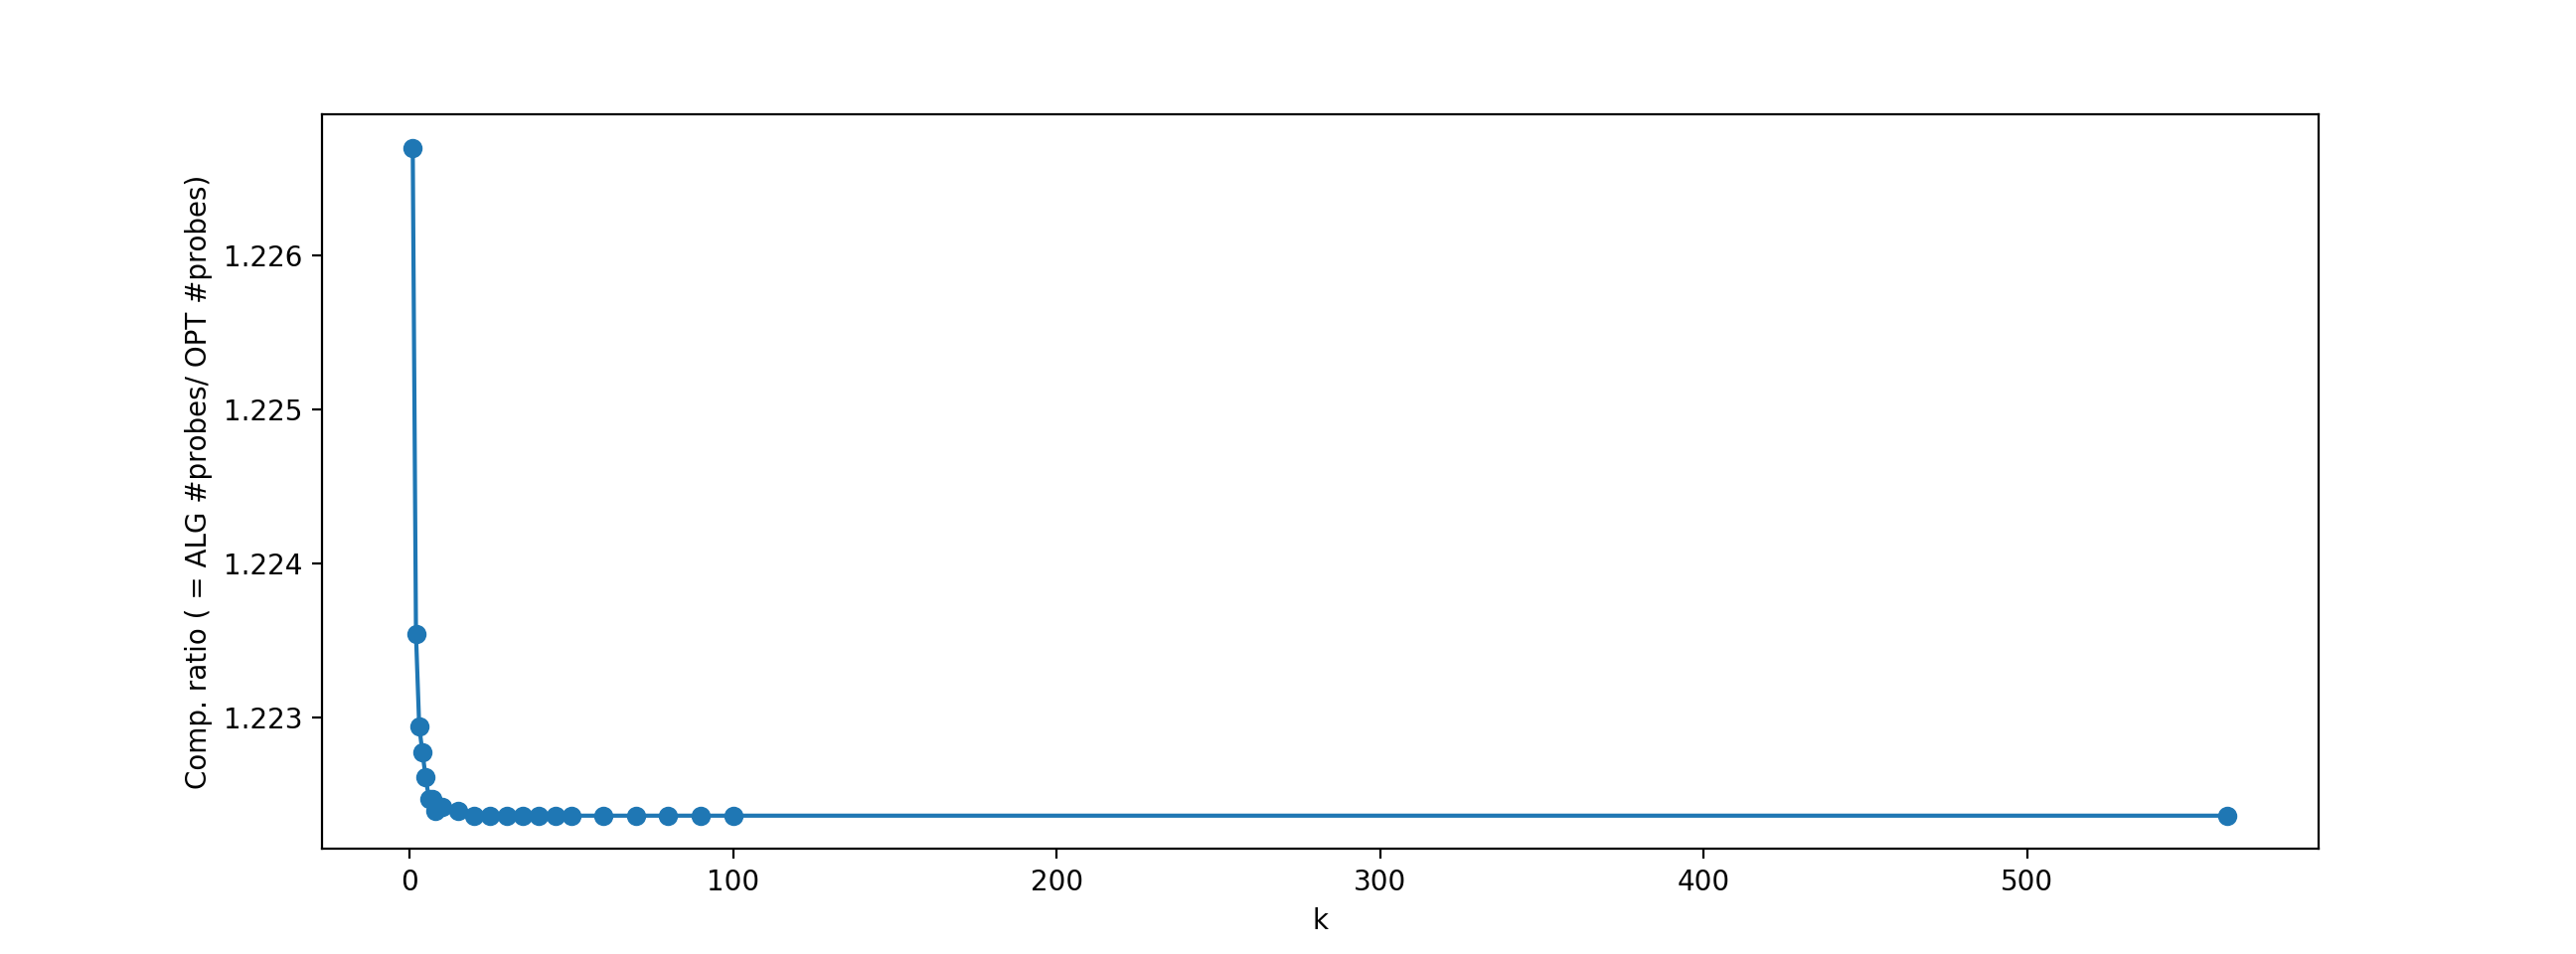
\includegraphics[width=0.9\textwidth,keepaspectratio]{cr-wide}
        %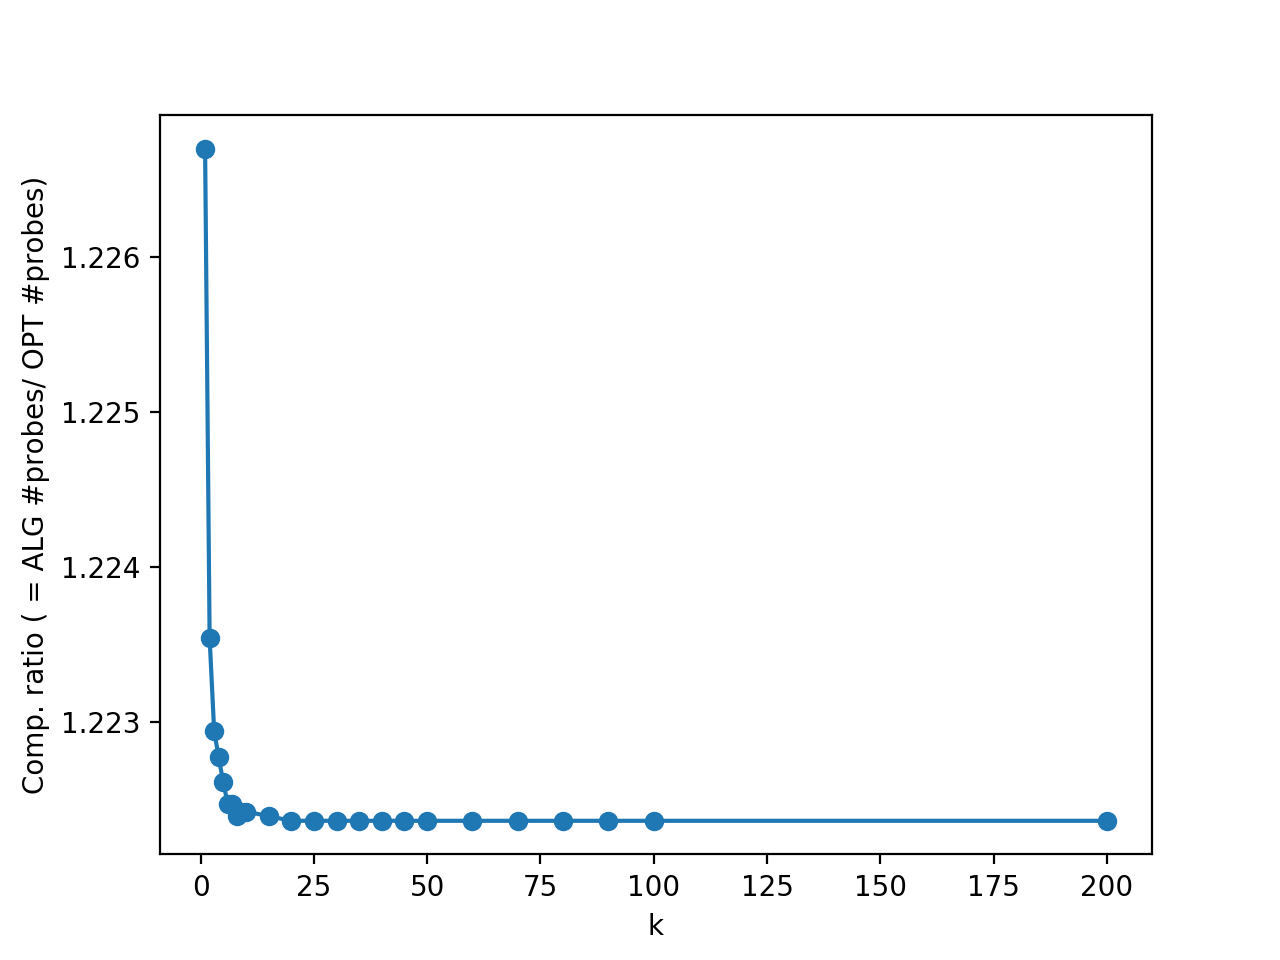
\includegraphics[width=0.9\textwidth,keepaspectratio]{cr-k-uniform}
    }   

    \quad
    
    \subfloat[]{
        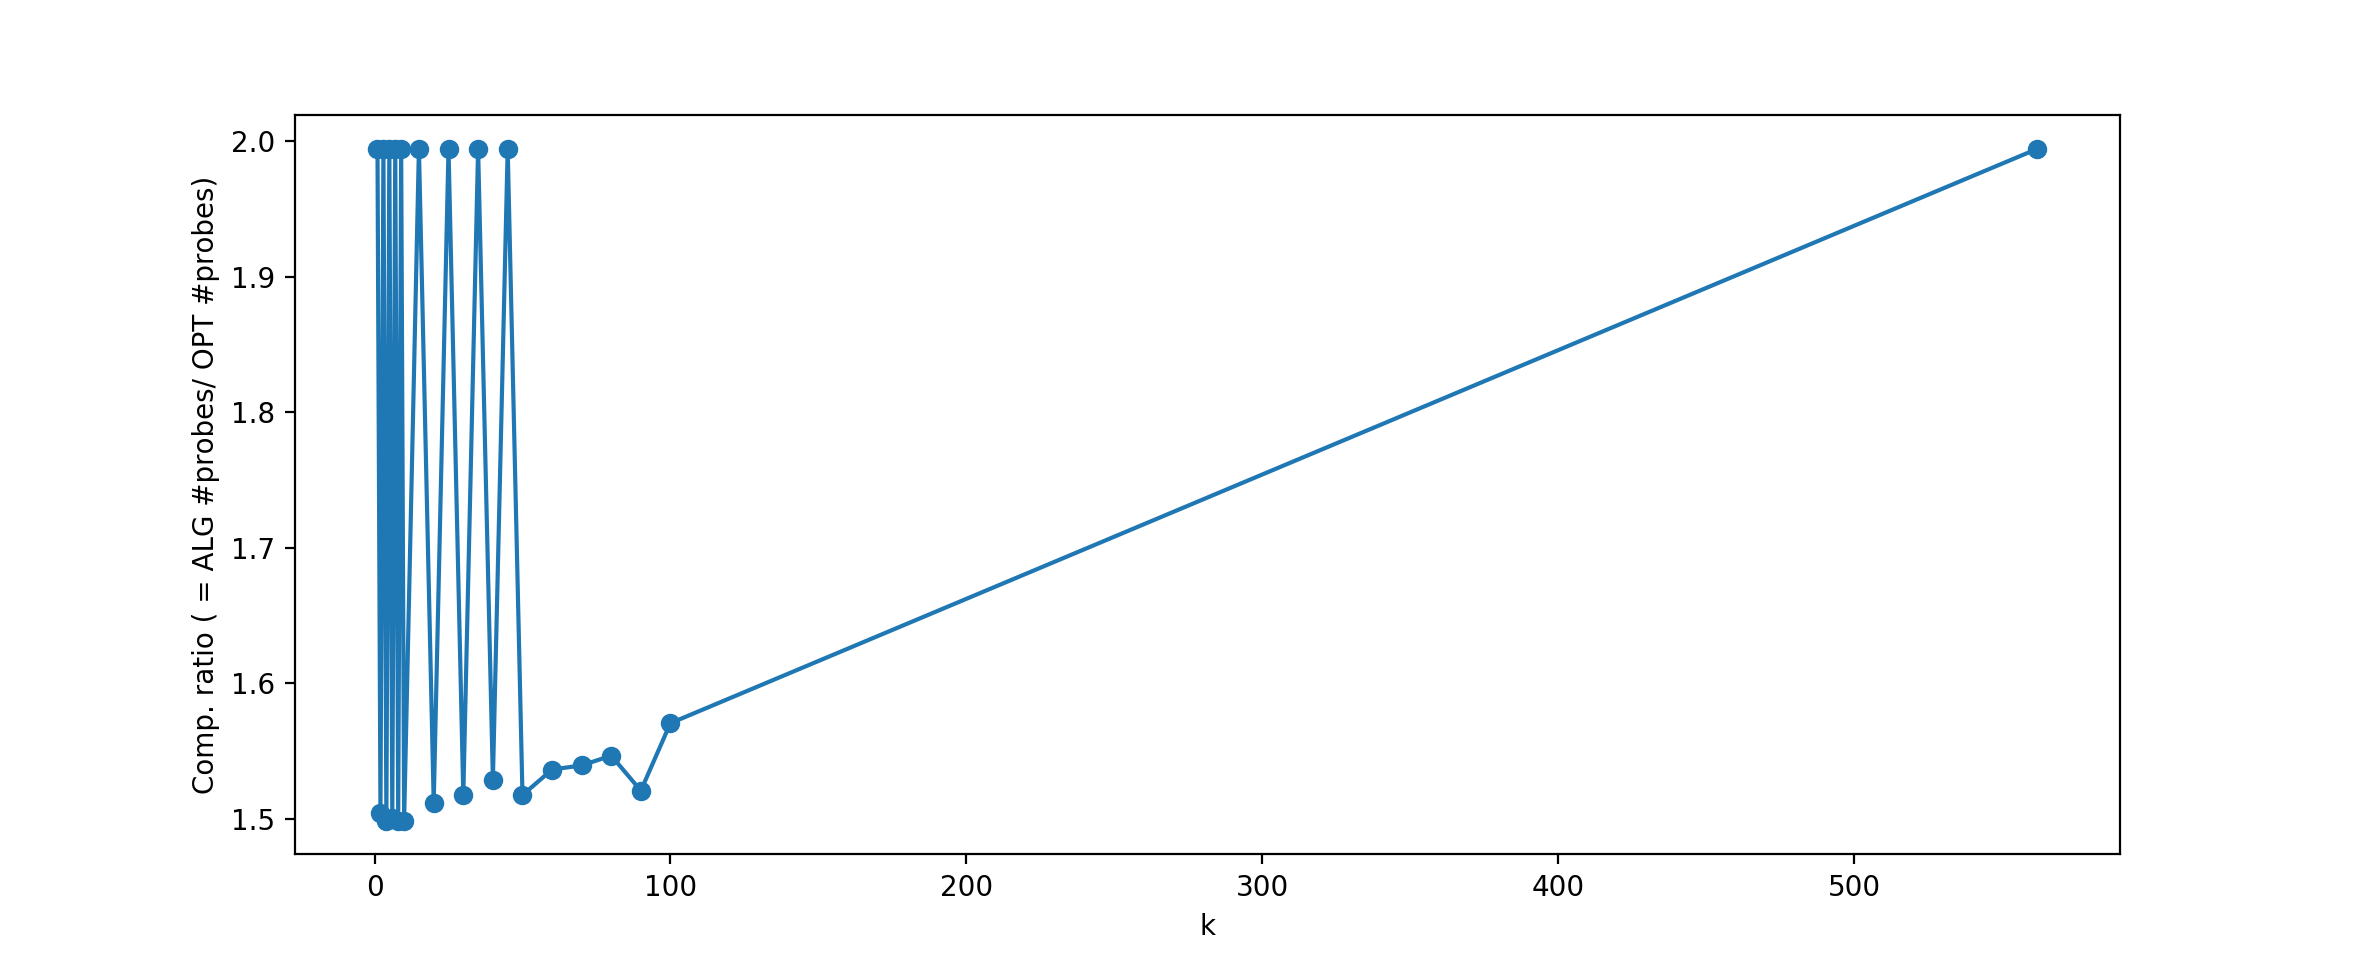
\includegraphics[width=0.9\textwidth,keepaspectratio]{cr-adversary-wide}
        %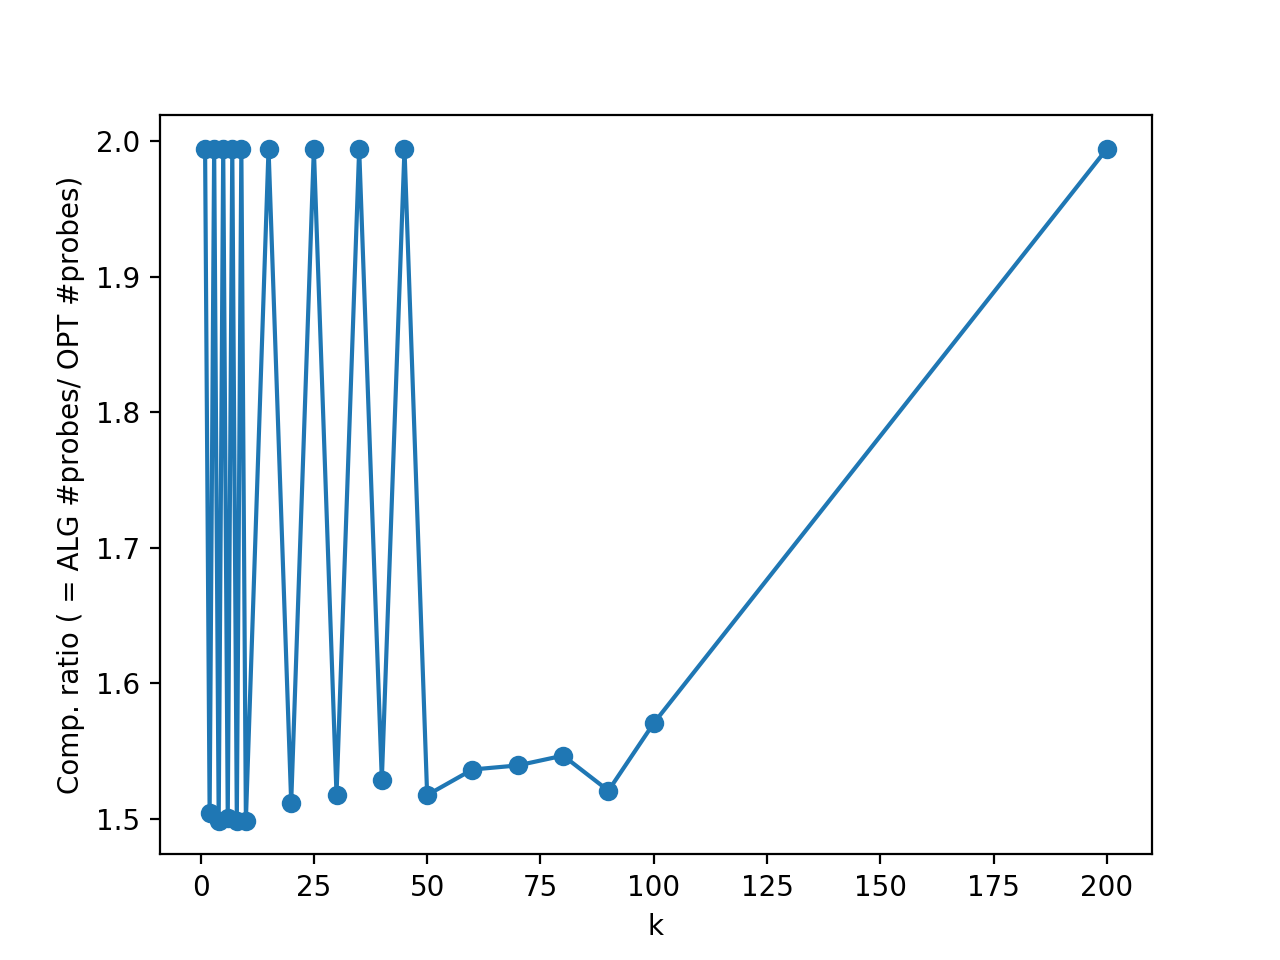
\includegraphics[width=0.9\textwidth,keepaspectratio]{cr-k-skewed}
    }
    \caption{The competitive ratios of LIP-$k$ against different $k$ values. We ran LIP-$k$ on uniform and adversarial datasets to produce (a) and (b) respectively. We plot $k = 1, 2, 3, 4, 5, 10, 15, 20, 25, 30, 35, 40, 45, 50, 60, 70, 80, 90, 100, 562$. The data point at $k = 562$ represents LIP (which is essentially LIP-$\infty$).}
    \label{fig:cr}
\end{figure}

When the keys in the fact table columns are distributed uniformly, the filters need not react to the local changes. LIP-$k$ with higher $k$produces a more accurate estimate of the selectivities than the LIP-$k$ with smaller $k$. Hence, the competitive ratio decreases slightly as $k$ increases, as depicted in Figure \ref{fig:cr}.

%@TODO: Explain the adversarial case using epsilons
Figure \ref{fig:cr}(b) displays how an adversarial dataset can make LIP-$k$ and LIP perform poorly. 
First, observe that LIP ({\it i.e.} LIP-562) achieves a competitive ratio of nearly 2.
Our modified query 4.2 has two joins, and thus the performance of LIP matches the worst case competitive ratio. 

LIP-$k$ with odd $k$ also achieves a competitive ratio of almost 2. 
For odd $k$, LIP-$k$'s selectivity estimates always contains one more odd (or even) batch than the other, 
and thus the estimated selectivity and filtering sequence are in favor of the majority batch type,
which produces the worst-case filter sequence on the following batch.

For even $k$, LIP-$k$'s selectivity estimates contain an equal amount of even an odd batches,  
and thus estimated selectivities remain the same ($1/2$ by construction) throughout the execution, 
and the filter sequence does not change. Thus for at most half of the batches it is optimal, 
and for the other half it is worse, 
resulting in a competitive ratio of at least \[ \frac{1 \times 1/2 + 2 \times 1/2}{1} = 1.5,\] as depicted in Figure \ref{fig:cr}. 

When $i \leq k$, LIP and LIP-$k$ execute identically, since LIP-$k$ has not yet ``forgotten" any previous batches. 
Thus, when $i \leq k$, LIP-$k$ achieves a competitive ratio of 2 on each batch, regardless of wheter $k$ is even or odd.
When $i > k$ and $k$ is odd, LIP-$k$ still achieves a competitive ratio of 2 on each batch.
However, When $i > k$ and $k$ is even, LIP-$k$ forgets to first batch and achieves a competive ratio of 1.5 on the remaining batches.
This explains why the competitive ratio increases for even $k$ as $k$ increases.
\footnote{An astute observer might notice that the competitive ratio decreases for $k = 50$ and $k = 90$. This is because the batch size is not constant throughout execution (see Section~\ref{sec:implementation}).}


%$k = 1, 2, 3, 4, 5, 10, 15, 20, 25, 30, 35, 40, 45, 50, 60, 70, 80, 90, 100$ on 


\section{Future Works}



\section{Concluding Remarks}

% concluding remarks below

The contributions of this project come in two-folds: We implemented Hash-join and LIP on top of Apache Arrow and thus provided an interface for future integration of Hustle on Apache Arrow; and we proposed LIP-$k$, a variant of LIP, which opens up an area for improving the performance LIP. It would also be interesting to study the problem of LIP in the online algorithmic setting to design an efficient mechanism utilizing randomness with better worst case guarantees. 


% Future work below

% In this work, there exists an adversarial fact table for all variants of LIP have that would force the algorithm to achieve a competitive ratio of $n$. However, reasonable applications of some existing random online algorithm mechanisms may yield a competitive ratio of $O(\log n)$ using the weighted majority algorithm \cite{littlestone1994weighted}. However, multiplicative updates on the weights may change the weighted average filter to use, but will not change the sequence of all filters if only comparing them based on their weights. More work is required here to either provide a mechanism to achieve a better competitive ratio, or provide a lower bound reduction showing that the competitive ratio of $n$ is tight even for random mechanisms.


\section*{Acknowledgements}

The authors wish to thank Prof.\ Jignesh Patel for constant feedbacks on this project and Kevin Gaffney for helping us with Apache Arrow specifics. The second author wishes to thank Prof.\ Paris Koutris for the suggestion of working on a practical project when the lemma production pipe is jammed. It works.


\bibliography{rep}{}
\bibliographystyle{plain}

\end{document}
